\documentclass[nobib]{tufte-handout}
\usepackage{etex} \reserveinserts{36}
\usepackage{graphicx}
\usepackage{morefloats}
\usepackage{cite}
\setkeys{Gin}{width=\linewidth,totalheight=\textheight,keepaspectratio}
\graphicspath{{figures/}}

% The units package provides nice, non-stacked fractions and better spacing
% for units.
% \usepackage{units}

% The fancyvrb package lets us customize the formatting of verbatim
% environments.  We use a slightly smaller font.
\usepackage{fancyvrb}
\fvset{fontsize=\normalsize}

% Small sections of multiple columns
% \usepackage{multicol}

% Brief personal statement addressing current research, professional contributions, and future goals



\hypersetup{colorlinks}

\newcommand{\minisec}[1]{\vspace{3pt} \noindent \emph{#1}\ }

\title{Research statement}
\author{\href{http://matsen.fredhutch.org/}{Frederick A. Matsen}, Fred Hutchinson Cancer Research Center}


\begin{document}

\maketitle

\begin{abstract}
\noindent
As large biological data sets become easily available, methodological advances in computational biology can greatly improve our understanding of hidden processes.
I am committed to building rigorous computational methods to solve important problems in biology and to making those tools accessible to biologists.
Guided by collaborative work on hard problems in biomedicine, I develop sequence analysis methods that integrate relevant biological details, that deliver meaningful uncertainty estimates, and that scale to large data sets.


\vspace{0.15cm}

\noindent
In the last five years, we begun a transition from making inferences under classical probabilistic models using classical techniques, to our next phase: making inferences under models without easily computed likelihoods, as well as developing next-generation inferential tools such as variational Bayes phylogenetic inference.
In the next five years, we will develop
\begin{enumerate}
\item variational Bayesian phylogenetic inference into an efficient, feature-rich, and complete inferential method
\item neural-network-based methods to study B cell somatic hypermutation and T cell receptor sequence diversity.
\end{enumerate}
\end{abstract}

\begin{marginfigure}[0.8in]%
  \includegraphics[width=1.95in]{bayesian_phylo}
  \caption{\
The objective of Bayesian phylogenetic inference is to infer a posterior distribution on phylogenetic trees, giving the probability that each of these trees is correct given some sequence data.
    }
  \label{FIGbayesPhylo}
\end{marginfigure}%


\vspace{0.3cm}
\subsection{Next-generation methods for Bayesian phylogenetic inference}
\vspace{-0.3cm}
The goal of Bayesian phylogenetic inference is to infer a posterior distribution on evolutionary trees given some sequence data (Figure~\ref{FIGbayesPhylo}).
Because sequence data and evolutionary signal is sparse for our domain of interest (pathogens and B cell receptors), and phylogenetic models are complex, there is considerable uncertainty in phylogenetic inferences.
Bayesian methods directly report that uncertainty, and make it possible to pass the uncertainty on to another phase of the analysis.
For example, we have found in collaborative work with the Overbaugh lab \cite{Simonich2019-nn} that B cell receptor phylogenetic trees show substantial uncertainty in their structure and ancestral sequences.
We want to make such probabilistic analysis much more efficient so that incorporating uncertainty becomes in integral part of evolutionary sequence analysis.

\begin{marginfigure}[-0.in]%
  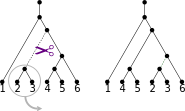
\includegraphics[width=1.95in]{spr-definition}
  \caption{\
    A phylogenetic tree and the result of applying a subtree-prune-regraft (SPR) modification to it.
    In this modification, a subtree is cut off the larger tree, then reattached using a new edge (dotted line of right hand tree).
    }
  \label{FIGsprdef}
\end{marginfigure}%

\newthought{Current Bayesian phylogenetic methods do not scale} to modern data sets.
These methods are based on the classical Markov chain Monte-Carlo (MCMC) algorithm, which performs random tree modifications (Figure~\ref{FIGsprdef}) whereby modifications that result in better (higher likelihood) trees are favored over jumps to worse trees.
However, most of these random modifications will result in a significantly worse tree, and thus are not accepted by the algorithm.
Such low acceptance rates directly prevent MCMC from working on large data.

In the past five years we have been obsessed with finding a scalable alternative to MCMC, applying
sequential Monte Carlo \cite{Dinh2017-sh,Fourment2017-an,Claywell2018-zg},
Hamiltonian Monte Carlo \cite{Dinh2017-oj},
systematic search \cite{Whidden2018-db} with efficient marginal likelihood estimation \cite{Fourment2018-xx},
and variational inference \cite{Zhang2018-lw,Zhang2018-mm}.
Of these, we will only continue to pursue variational inference.

\begin{marginfigure}[0.in]%
  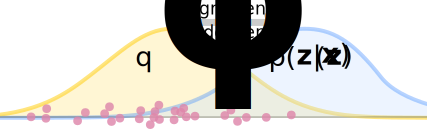
\includegraphics[width=1.95in]{variational-gradient}
  \caption{\
    Variational inference fits an approximating distribution $q_\phi$ to the posterior $p$ by modifying parameters $\phi$.
    Pink circles schematize samples from the current approximate posterior; having these samples in hand enables efficient gradient descent steps to fit $q_\phi$.
    }
  \label{FIGvariationalGradient}
\end{marginfigure}%

Variational inference is an alternative approach to posterior inference that fits a so-called variational approximation to a posterior distribution (Figure~\ref{FIGvariationalGradient}).
Accurate variational inference methods depend on a variational approximation that can closely match the true posterior distribution.
We perform variational inference on the set of phylogenetic trees, an intricate mixture of discrete and continuous aspects for which it is not at all obvious how to parameterize a distribution using real-valued parameters.

\begin{marginfigure}[0.7in]%
  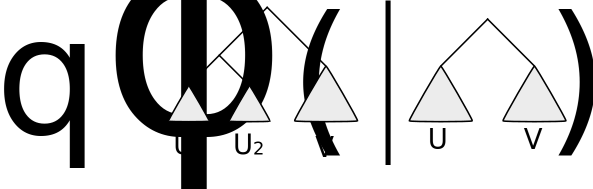
\includegraphics[width=1.95in]{csd}
  \caption{\
    A tree topology can be broken down into a collection of conditional statements about splitting of subtrees.
    Our variational parameterization on tree topologies approximates a posterior on tree topologies as a product of conditional probabilities about these splitting steps.
    }
  \label{FIGcsd}
\end{marginfigure}%

Our variational inference method is in terms of conditional probabilities of splitting events on trees (Figure~\ref{FIGcsd}).
We have shown that such a parameterization is sufficiently rich to capture the structure of real phylogenetic posterior distributions \cite{Zhang2018-mm}.
In fact, we showed that simply fitting such a distribution to an MCMC sample of phylogenetic trees results in a better approximation to the posterior than simply using the MCMC samples, showing that the ``information sharing'' inherent in our parameterization smooths out the stochasticity inherent in an MCMC sample.

\begin{marginfigure}[0.7in]%
  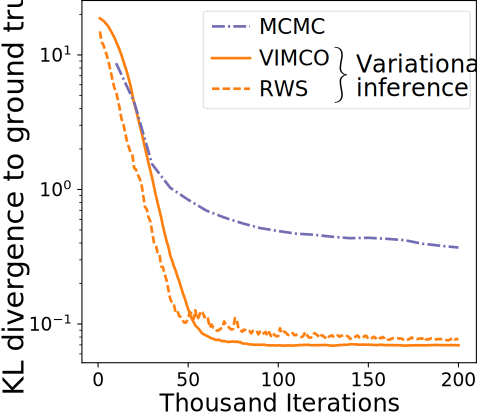
\includegraphics[width=1.95in]{vbpi-performance}
  \caption{\
    The performance of direct variational Bayes phylogenetic inference on benchmark data set DS1 (lower is better).
    }
  \label{FIGvbpiPerformance}
\end{marginfigure}%

We then combined this variational parameterization on phylogenetic tree topologies with a parameterization on tree branch lengths to obtain a complete parameterization on phylogenetic trees, which enables direct variational inference from data \cite{Zhang2018-lw}.
We showed that our variational methods quickly approximate the posterior (Figure~\ref{FIGvbpiPerformance}).

\paragraph{The future}
We are moving quickly to ensure variational Bayesian inference will achieve its promise.
This includes developing \href{https://github.com/matsengrp/libsbn/}{libsbn}, a Python-interface C++ library to provide efficient implementation of variational Bayes phylogenetic inference and enable researchers to develop phylogenetic models using Python-based modeling platforms such as \href{https://www.tensorflow.org/}{Tensorflow} and \href{https://pytorch.org/}{PyTorch}.
This package will allow us to specify and do inference on complex phylogenetic models.
We are also developing methods to allow divide-and-conquer Bayesian phylogenetic inference, which we believe is an essential component of scaling phylogenetic inference to large data sets.
Farther down the road, we also believe that variational methods can enable whole-sequence-based phylogenetic inference methods, which will allow us to avoid the ubiquitous independence-across-sites assumption.

\newpage
\bibliography{main}
\bibliographystyle{tufte}

\end{document}
